\begin{XeClass}{RawLocalFileSystem}
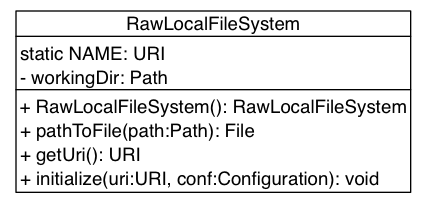
\includegraphics[width=\textwidth]{cdig/RawLocalFileSystem.png}
     
 该类实现了一个原生本地文件系统。可以作为一个具有最基本功能的文件系统。

    \begin{XeMethod}{\XePublic}{RawLocalFileSystem}{RawLocalFileSystem}
         
 在构造方法中完成对用户的当前工作目录的初始化

    \end{XeMethod}

    \begin{XeMethod}{\XePublic}{File}{pathToFile}
         
 Convert a path to a File.
 用于将一个路径转化为以用户工作目录为父目录的绝对路径

    \end{XeMethod}

    \begin{XeMethod}{\XePublic}{URI}{getUri}
         
 获取本地文件名的URI

    \end{XeMethod}

    \begin{XeMethod}{\XePublic}{void}{initialize}
         
 初始化

    \end{XeMethod}

    \begin{XeInnerClass}{TrackingFileInputStream}
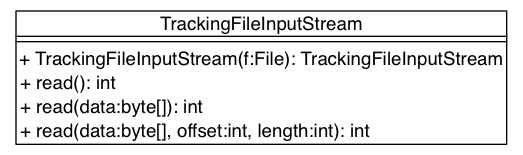
\includegraphics[width=\textwidth]{cdig/TrackingFileInputStream.png}
         
 本地文件系统的读取操作
 会将读到的字节数添加到统计信息中

    \end{XeInnerClass}
    \begin{XeInnerClass}{LocalFSFileInputStream}
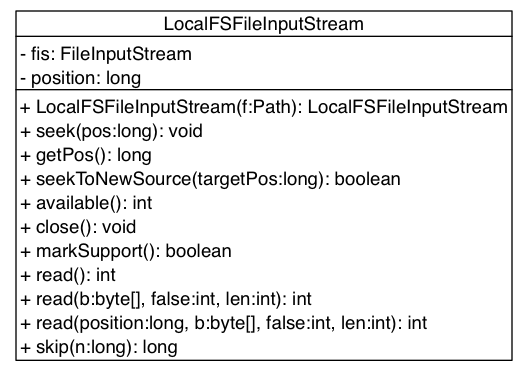
\includegraphics[width=\textwidth]{cdig/LocalFSFileInputStream.png}
         
 依靠包装的FileInputStream的实例进行读取操作
 通过 TrackingFileInputStream来初始化

    \end{XeInnerClass}
    \begin{XeInnerClass}{LocalFSFileOutputStream}
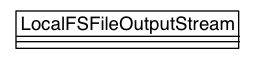
\includegraphics[width=\textwidth]{cdig/LocalFSFileOutputStream.png}
         
 For create()'s FSOutputStream.
 同输入流,依靠包装的FileOutputStream的实例进行写入操作

    \end{XeInnerClass}

\end{XeClass}
